

\section{La geometría de los triángulos: congruencia, similitud y el teorema de Pitágoras}

\subsection{Triángulos congruentes}

{}
	Los triángulos que tienen el mismo tamaño y la misma forma se llaman \emph{triángulos congruentes}.

{}
	\begin{center}
		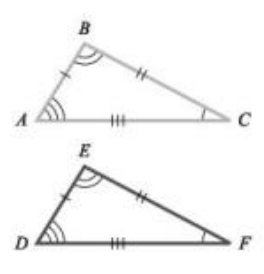
\includegraphics[height=8cm,keepaspectratio=true]{./trig/algsup3-01.png}
		% algsup3-01.png: 0x0 pixel, 300dpi, 0.00x0.00 cm, bb=
	\end{center}
	

{}
	Si dos triángulos $\triangle ABC, \triangle DEF$ son congruentes, escribiremos \begin{align*}
		\triangle ABC \cong \triangle DEF.
	\end{align*}

{}
	\begin{prop}[Criterios de congruencia]
		\begin{itemize}
			\item \emph{LAL}: Dos lados y su ángulo incluido iguales.
			\item \emph{ALA}: Dos ángulos y su lado incluido iguales. 
			\item \emph{LLL}: Tres lados iguales. 
		\end{itemize}
		
	\end{prop}
	


\subsection{Triángulos semejantes}
[t]{}
	\begin{wrapfigure}[15]{l}{5cm}
		%%%%%%%%%%%%%%%%%%%%%%%%%%%%%%%%%%%%%%%%%%%%%%%%%%%%%%%%%%%%%%%%%%%%%%%%%%%%%%%%%%%%%%%
		%%% You will need to add \usepackage{wrapfig} to your preamble to use textwrapping %%%
		%%%%%%%%%%%%%%%%%%%%%%%%%%%%%%%%%%%%%%%%%%%%%%%%%%%%%%%%%%%%%%%%%%%%%%%%%%%%%%%%%%%%%%%
		\centering
		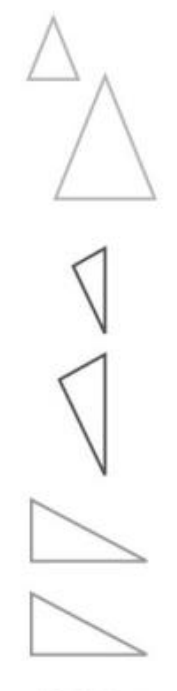
\includegraphics[width=2cm,keepaspectratio=true]{./trig/algsup3-02.png}
		% algsup3-02.png: 0x0 pixel, 300dpi, 0.00x0.00 cm, bb=
		\label{fig:3-02}
	\end{wrapfigure}
	
	Diremos que dos triángulos $\triangle ABC$ y $\triangle DEF$ son \emph{similares} si 
	existe un correspondencia $A\leftrightarrow D, B\leftrightarrow E, C \leftrightarrow F$
	tal que $\frac{|AB|}{|DE|}=\frac{|BC|}{|EF|}=\frac{|CA|}{|FD|}=: \alpha.$
	
	
	A tal \emph{constante de proporcionalidad} $\alpha$ se conoce como \emph{escala}.

{}
	\begin{prop}[Criterio \emph{AA}]
		Si las medidas de dos ángulos de un triángulo son iguales a las de dos ángulos correspondientes de un segundo triángulo, entonces los dos triángulos son semejantes.
	\end{prop}
	

[t]{}
	\begin{problema}
		\label{exmp:9405}
		\begin{wrapfigure}[15]{L}{6cm}
			%%%%%%%%%%%%%%%%%%%%%%%%%%%%%%%%%%%%%%%%%%%%%%%%%%%%%%%%%%%%%%%%%%%%%%%%%%%%%%%%%%%%%%%
			%%% You will need to add \usepackage{wrapfig} to your preamble to use textwrapping %%%
			%%%%%%%%%%%%%%%%%%%%%%%%%%%%%%%%%%%%%%%%%%%%%%%%%%%%%%%%%%%%%%%%%%%%%%%%%%%%%%%%%%%%%%%
			\centering
			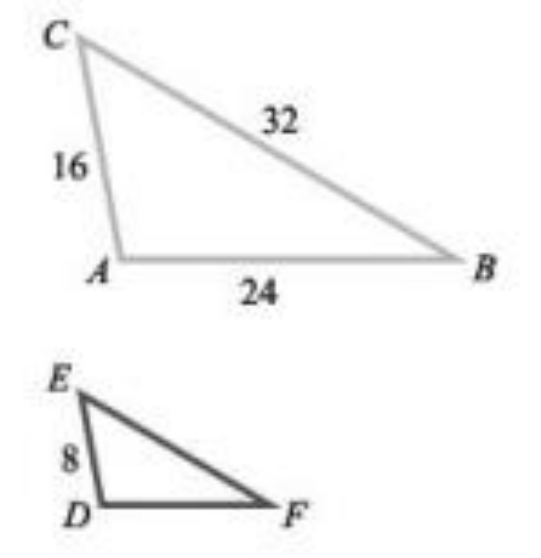
\includegraphics[width=5cm,keepaspectratio=true]{./trig/trig9446.png}
			% trig9446.png: 0x0 pixel, 300dpi, 0.00x0.00 cm, bb=
			\label{fig:9446}
		\end{wrapfigure}
		Suponga que en la figura, ambos triángulos son semejantes. Encuentre las longitudes desconocidas de los lados de $\triangle EDF.$
	\end{problema}
	

[t]{}
	\begin{problema}
		\label{exmp:9406}
		\begin{wrapfigure}[15]{L}{6cm}
			%%%%%%%%%%%%%%%%%%%%%%%%%%%%%%%%%%%%%%%%%%%%%%%%%%%%%%%%%%%%%%%%%%%%%%%%%%%%%%%%%%%%%%%
			%%% You will need to add \usepackage{wrapfig} to your preamble to use textwrapping %%%
			%%%%%%%%%%%%%%%%%%%%%%%%%%%%%%%%%%%%%%%%%%%%%%%%%%%%%%%%%%%%%%%%%%%%%%%%%%%%%%%%%%%%%%%
			\centering
			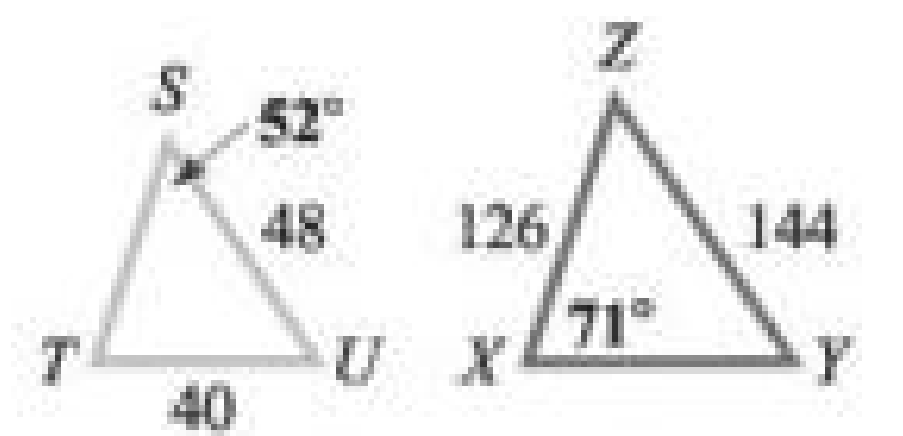
\includegraphics[width=5cm,keepaspectratio=true]{./trig/trig9447.png}
			% trig9446.png: 0x0 pixel, 300dpi, 0.00x0.00 cm, bb=
			\label{fig:9447}
		\end{wrapfigure}
		Encuentre las medidas de las partes desconocidas de los triángulos semejantes $\triangle STU$ y $\triangle ZXY.$ 
	\end{problema}
	

[t]{}
	\begin{problema}
		\label{exmp:9407}
		\begin{wrapfigure}[15]{L}{6cm}
			%%%%%%%%%%%%%%%%%%%%%%%%%%%%%%%%%%%%%%%%%%%%%%%%%%%%%%%%%%%%%%%%%%%%%%%%%%%%%%%%%%%%%%%
			%%% You will need to add \usepackage{wrapfig} to your preamble to use textwrapping %%%
			%%%%%%%%%%%%%%%%%%%%%%%%%%%%%%%%%%%%%%%%%%%%%%%%%%%%%%%%%%%%%%%%%%%%%%%%%%%%%%%%%%%%%%%
			\centering
			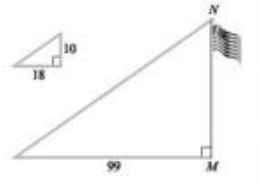
\includegraphics[width=5cm,keepaspectratio=true]{./trig/trig9448.png}
			% trig9446.png: 0x0 pixel, 300dpi, 0.00x0.00 cm, bb=
			\label{fig:9448}
		\end{wrapfigure}
		La jefa de oficina de correos de una ciudad quiere medir la altura del asta de la bandera de la oficina. Observa que en el instante en el que la sombra de la estación mide $18fts$, la sombra del asta mide $99fts$. El edificio tiene $10fts$ de altura. ¿Cuál es la altura del asta?
	\end{problema}
	

\subsection{El teorema de Pitágoras}
{}
	\begin{thm}[Pitágoras]
		\begin{wrapfigure}[10]{L}{6cm}
			%%%%%%%%%%%%%%%%%%%%%%%%%%%%%%%%%%%%%%%%%%%%%%%%%%%%%%%%%%%%%%%%%%%%%%%%%%%%%%%%%%%%%%%
			%%% You will need to add \usepackage{wrapfig} to your preamble to use textwrapping %%%
			%%%%%%%%%%%%%%%%%%%%%%%%%%%%%%%%%%%%%%%%%%%%%%%%%%%%%%%%%%%%%%%%%%%%%%%%%%%%%%%%%%%%%%%
			\centering
			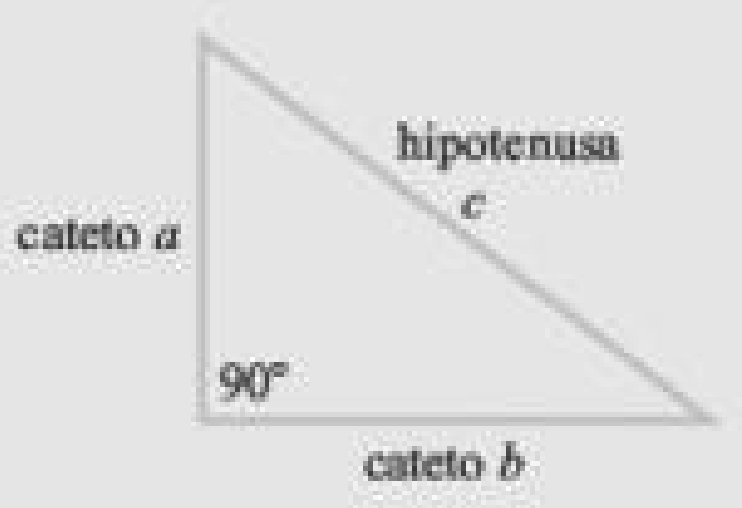
\includegraphics[width=5cm,keepaspectratio=true]{./trig/trig94thm.png}
			% trig94thm.png: 0x0 pixel, 300dpi, 0.00x0.00 cm, bb=
			\label{fig:94thm}
		\end{wrapfigure}
		\begin{align*}
			a^{2}+b^{2}=c^{2}
		\end{align*}
	\end{thm}
	

{}
	Los números naturales $\set{3,4,5}$ forman una \emph{terna pitagórica}, ya que satisfacen las ecuaciones del teorema de Pitágoras. 

[t]{}
	\begin{problema}
		\label{exmp:9408}
		\begin{wrapfigure}[5]{l}{5cm}
			%%%%%%%%%%%%%%%%%%%%%%%%%%%%%%%%%%%%%%%%%%%%%%%%%%%%%%%%%%%%%%%%%%%%%%%%%%%%%%%%%%%%%%%
			%%% You will need to add \usepackage{wrapfig} to your preamble to use textwrapping %%%
			%%%%%%%%%%%%%%%%%%%%%%%%%%%%%%%%%%%%%%%%%%%%%%%%%%%%%%%%%%%%%%%%%%%%%%%%%%%%%%%%%%%%%%%
			\centering
			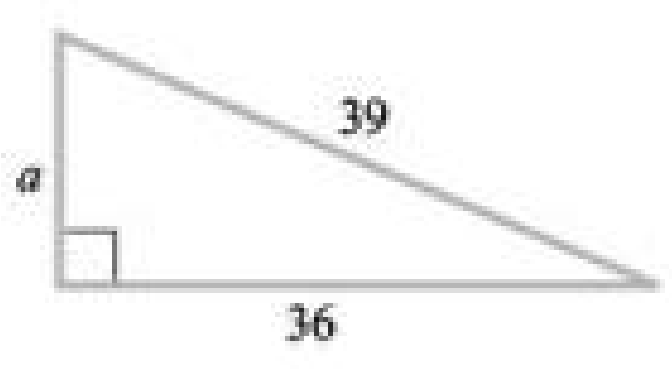
\includegraphics[width=5cm,keepaspectratio=true]{./trig/trig9450.png}
			% trig9450.png: 0x0 pixel, 300dpi, 0.00x0.00 cm, bb=
			\label{fig:9450}
		\end{wrapfigure}
		
		Determine la longitud $a$ del triángulo rectángulo que se muestra.
	\end{problema}
	

[t]{}
	\begin{problema}
		\label{exmp:9409}
		\begin{wrapfigure}[5]{l}{5cm}
			%%%%%%%%%%%%%%%%%%%%%%%%%%%%%%%%%%%%%%%%%%%%%%%%%%%%%%%%%%%%%%%%%%%%%%%%%%%%%%%%%%%%%%%
			%%% You will need to add \usepackage{wrapfig} to your preamble to use textwrapping %%%
			%%%%%%%%%%%%%%%%%%%%%%%%%%%%%%%%%%%%%%%%%%%%%%%%%%%%%%%%%%%%%%%%%%%%%%%%%%%%%%%%%%%%%%%
			\centering
			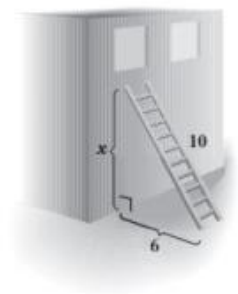
\includegraphics[width=5cm,keepaspectratio=true]{./trig/trig9451.png}
			% trig9450.png: 0x0 pixel, 300dpi, 0.00x0.00 cm, bb=
			\label{fig:9451}
		\end{wrapfigure}
		Una escalera de 10 metros de longitud tiene su base a 6 metros de la pared. ¿Qué altura alcanza la escalera?
	\end{problema}
	


\section{Los ángulos y sus medidas}
\subsection{Terminología básica}
{}
	\begin{figure}[h]
		\centering
		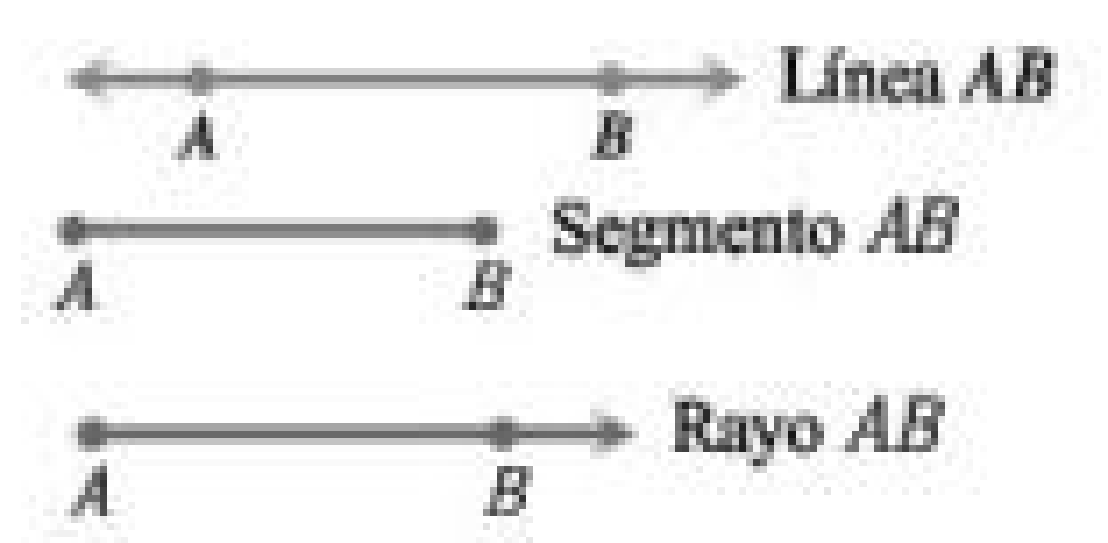
\includegraphics[width=10cm,keepaspectratio=true]{./trig/trig_101-1.png}
		% trig_10.1-1.png: 0x0 pixel, 300dpi, 0.00x0.00 cm, bb=
		\label{fig:101-1}
	\end{figure}
	

{}
	\begin{figure}[h]
		\centering
		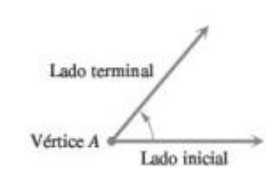
\includegraphics[width=10cm,keepaspectratio=true]{./trig/trig_101-2.png}
		% trig_10.1-1.png: 0x0 pixel, 300dpi, 0.00x0.00 cm, bb=
		\label{fig:101-2}
	\end{figure}
	

{}
	\begin{figure}[h]
		\centering
		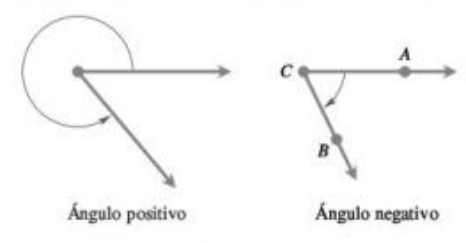
\includegraphics[width=10cm,keepaspectratio=true]{./trig/trig_101-3.png}
		% trig_10.1-1.png: 0x0 pixel, 300dpi, 0.00x0.00 cm, bb=
		\label{fig:101-3}
	\end{figure}
	

{}
	\begin{figure}[h]
		\centering
		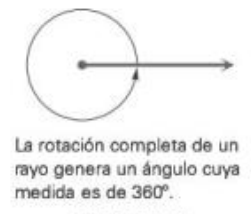
\includegraphics[width=10cm,keepaspectratio=true]{./trig/trig_101-4.png}
		% trig_10.1-1.png: 0x0 pixel, 300dpi, 0.00x0.00 cm, bb=
		\label{fig:101-4}
	\end{figure}
	

{}
	\begin{figure}[h]
		\centering
		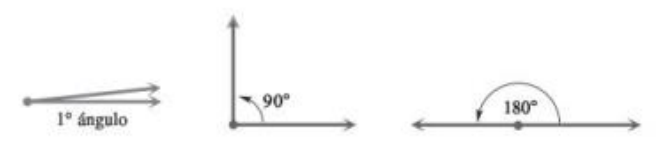
\includegraphics[width=10cm,keepaspectratio=true]{./trig/trig_101-5.png}
		% trig_10.1-1.png: 0x0 pixel, 300dpi, 0.00x0.00 cm, bb=
		\label{fig:101-5}
	\end{figure}
	

{}
	\begin{figure}[h]
		\centering
		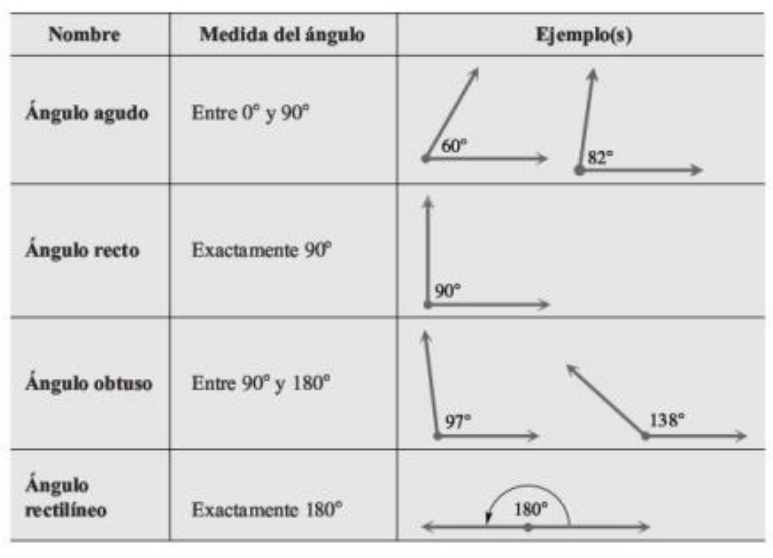
\includegraphics[width=8cm,keepaspectratio=true]{./trig/trig_101-tab1.png}
		% trig_101-tab1.png: 0x0 pixel, 300dpi, 0.00x0.00 cm, bb=
		\label{fig:101-tab1}
	\end{figure}
	

{}
	Si la suma de las medidas de  dos ángulos es $90^{o},$ los ángulos se llaman \emph{complementarios}. En tanto que dos ángulos cuyas medidas sumen $180^{o}$ son \emph{suplementarios}.

{}
	\begin{problema}
		\label{exmp:1011}
		Diga cuál es el complemento y el suplemento de $50^{o}$.
	\end{problema}
	

\subsection{Radianes}
{}
	Un \emph{ángulo central} es un ángulo positivo cuyo vértice esta en el centro de un círculo. 

{}
	\begin{figure}[h]
		\centering
		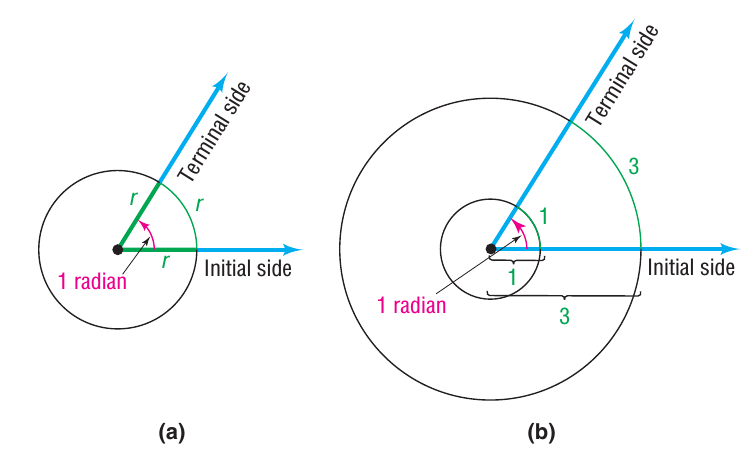
\includegraphics[height=5cm,keepaspectratio=true]{./trig/sull0610.png}
		% sull0610.png: 0x0 pixel, 300dpi, 0.00x0.00 cm, bb=
		\label{fig:sull6110}
	\end{figure}
	

{}
	\begin{thm}[Longitud de arco]
		Para un círculo de radio $r$, un ángulo central  de $\theta$ radianes subtiende un arco cuya longitud es 
		\begin{align}
			\label{sull6104}
			s = r\theta
		\end{align}
	\end{thm}
	

{}
	\begin{problema}
		\label{exmp:sull6103}
		Encuentre la longitud de arco de un círculo de radio $2$ subtendido por un ángulo central de $0.25$ radianes. 
	\end{problema}

{}
	\begin{problema}
		\label{exe:sull6171}
		Encuentre la longitud de arco de un círculo de radio $10$ subtendido por un ángulo central de $\frac{1}{2}$ radianes. 
	\end{problema}
	

\subsection{Conversión entre grados y radianes}
{}
	\begin{figure}[h]
		\centering
		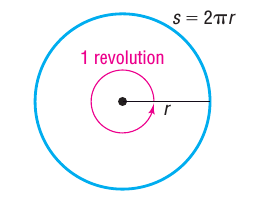
\includegraphics[height=5cm,keepaspectratio=true]{./trig/sull6112.png}
		% sull6112.png: 0x0 pixel, 300dpi, 0.00x0.00 cm, bb=
		\label{fig:sull6112}
		\caption{1 revolución = $2\pi$ radianes}
	\end{figure}
	

{}
	Como una revolución equivale a $360^{o},$ entonces $1 \texttt{rad}=360^{0}.$ De manera simplificada:
	\begin{align*}
		180^{o}= \pi\texttt{rad}
	\end{align*}

{}
	\begin{problema}
		Convierta cada uno de los ángulos a radianes:
		\begin{itemize}
			\item $60^{o}=$ 
			\item $150^{o}=$ 
			\item $-45^{o}=$ 
			\item $90^{o}=$ 
			\item $107^{o}$ 
		\end{itemize}
		
	\end{problema}
	

{}
	\begin{problema}
		\begin{itemize}
			\item Convierta $35^{o}$ a radianes, expresándolo como un múltiplo de $\pi$.
			\item Convierta $-40^{o}$ a radianes, expresándolo en decimales. 
		\end{itemize}
		
	\end{problema}
	

{}
	\begin{figure}[h]
		\centering
		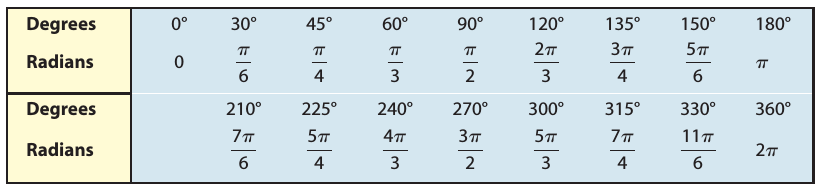
\includegraphics[width=10cm,keepaspectratio=true]{./trig/sull61t1.png}
		% sull61t1.png: 0x0 pixel, 300dpi, 0.00x0.00 cm, bb=
		\label{fig:61t1}
	\end{figure}
	

{}
	\begin{problema}
		La latitud de una locación $L$ es la medida del ángulo formado por un rayo dibujado desde el centro de la tierra al ecuador y un rayo dibujado del centro de la tierra a $L$. 
		
		Glasgow, Montana está al norte de Albuquerque, Nuevo México. Encuentre la distancia entre Glasgow, $48^{o}, 9'$, latitud Norte y Albuquerque, $35^{o}, 5'$. Suponga que el radio de la tierra es $3960$ millas.
	\end{problema}
	

{}
	\begin{figure}[h]
		\centering
		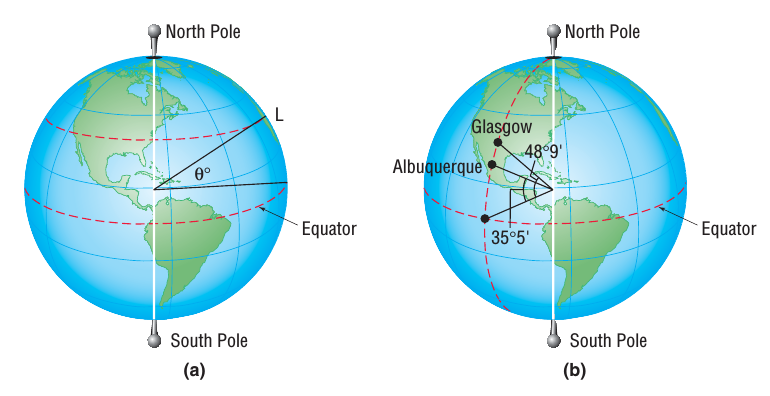
\includegraphics[width=10cm,keepaspectratio=true]{./trig/sull113.png}
		% sull113.png: 0x0 pixel, 300dpi, 0.00x0.00 cm, bb=
		\label{fig:sull6113}
	\end{figure}
	

{}
	\begin{problema}
		Memphis, Tennessee, está al norte de Nueva Orleans, Lousiana. Encuentre la distancia entre Memphis, $35^{o}, 9'$ latitud norte, y Nueva Orleans, $29^{o}, 57'$ latitud norte. Suponga que el radio de la tierra es $3960$ millas. 
	\end{problema}
	

\subsection{Área de un sector de un círculo} 
{}
	\begin{figure}[h]
		\centering
		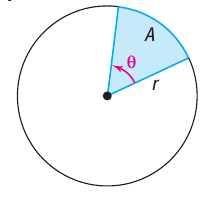
\includegraphics[height=5cm,keepaspectratio=true]{./trig/sull614.png}
		% sull614.png: 0x0 pixel, 300dpi, 0.00x0.00 cm, bb=
		\label{fig:sull6114}
	\end{figure}

{}
	\begin{figure}[h]
		\centering
		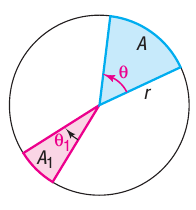
\includegraphics[height=5cm,keepaspectratio=true]{./trig/sull6115.png}
		% sull614.png: 0x0 pixel, 300dpi, 0.00x0.00 cm, bb=
		\label{fig:sull6115}
	\end{figure}

{}
	\begin{thm}[Área de un sector]
		El área $A$ de un sector de un círculo de radio $r$ formado por un ángulo central de $\theta$ radianes es 
		\begin{align}
			\label{sull6108}
			A=\frac{1}{2}r^{2}\theta.
		\end{align}
	\end{thm}
	

{}
	\begin{problema}
		\label{exmp:sull6107}
		Encuentre el área del sector de un círculo de radio $2fts$ formado por un ángulo de $30^{o}$. Redondee la respuesta dos decimales.  
	\end{problema}
	

{}
	\begin{problema}
		Encuentre el área del sector de un círculo de radio $10m$ formado por un ángulo de $\frac{1}{2}rad$. Redondee la respuesta dos decimales.  
	\end{problema}
	

\subsection{Movimiento circular}
{}
	\begin{figure}[h]
		\centering
		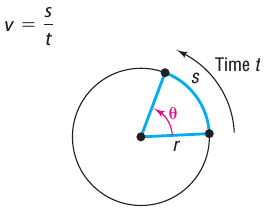
\includegraphics[height=5cm,keepaspectratio=true]{./trig/sull6116.png}
		% sull6116.png: 0x0 pixel, 300dpi, 0.00x0.00 cm, bb=
		\label{fig:sull6116}
	\end{figure}
	

{}
	Supongamos que un objeto se mueve alrededor de un círculo de radio $r$ a una rapidez constante. Si $s$ es la distancia recorrida en un tiempo $t$ alrededor del círculo, entonces la \emph{rapidez lineal} $v$ de este objeto se define como
	\begin{align}
		\label{sull6109}
		v=\dfrac{s}{t}
	\end{align}

{}
	La \emph{rapidez angular} $\om$ de este objeto es el ángulo $\theta$ (medido en radianes) barrido, dividido por el lapso $t$, es decir, 
	\begin{align}
		\label{sull6110}
		\om=\dfrac{\theta}{t}.
	\end{align}
	
	De manera que 
	\begin{align}
		\label{sull6111}
		v = r\om.
	\end{align}

{}
	\begin{wrapfigure}{l}{6cm}
		%%%%%%%%%%%%%%%%%%%%%%%%%%%%%%%%%%%%%%%%%%%%%%%%%%%%%%%%%%%%%%%%%%%%%%%%%%%%%%%%%%%%%%%
		%%% You will need to add \usepackage{wrapfig} to your preamble to use textwrapping %%%
		%%%%%%%%%%%%%%%%%%%%%%%%%%%%%%%%%%%%%%%%%%%%%%%%%%%%%%%%%%%%%%%%%%%%%%%%%%%%%%%%%%%%%%%
		\centering
		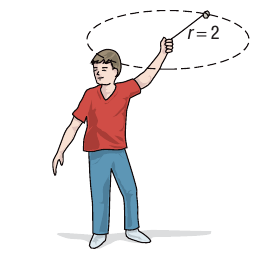
\includegraphics[width=5cm,keepaspectratio=true]{./trig/sull6117.png}
		% sull6117.png: 0x0 pixel, 300dpi, 0.00x0.00 cm, bb=
		\label{fig:6117}
	\end{wrapfigure}
	\begin{problema}
		\label{exmp:6108}
		Una persona está haciendo una roca atada al extremo de un cuerda de $2fts$ a un ritmo de $180rpm$. Encuentre la rapidez lineal de la roca en el instante en que es liberada.
	\end{problema}
	

{}
	\begin{problema}
		\label{exe:sull6197}
		Un objeto está viajando alrededor de un círculo de radio $5cm$. Si en $20s$ un ángulo central de $\dfrac{1}{3}rad$ es barrido, ¿cuál es su rapidez angular? ¿Cuál es su rapidez lineal?
	\end{problema}
	


	

\section{Funciones trigonométricas: El enfoque del círculo unitario}
\subsection{El círculo unitario}
{}
	\begin{figure}[h]
		\centering
		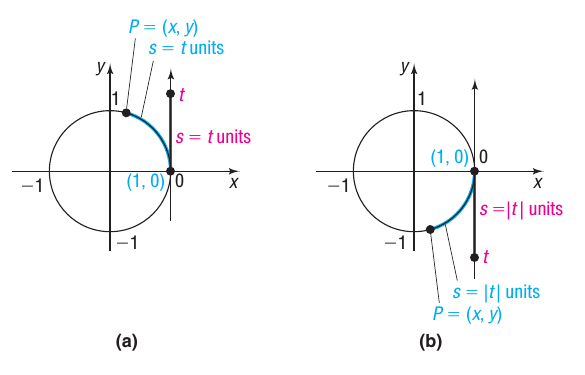
\includegraphics[width=10cm,keepaspectratio=true]{./trig/sull0618.png}
		% sull0618.png: 0x0 pixel, 300dpi, 0.00x0.00 cm, bb=
		\label{fig:0618}
	\end{figure}
	

{}
	\begin{defn}[Funciones trigonométricas]
		Sea $t$ un número real y $P=(x,y)$ el punto en el círculo unitario que corresponde a $t$.
		\begin{multicols}{2}
			\begin{itemize}
				\item $\sin(t)=y$
				\item $\cos(t)=x$
				\item $\tan(t)=\frac{y}{x}$
				\item $\csc(t)=\frac{1}{y}$
				\item $\sec(t)=\frac{1}{x}$
				\item $\cot(t)=\frac{x}{y}$
			\end{itemize}
		\end{multicols}
	\end{defn}

{}
	\begin{problema}
		\label{exmp:sull0601}
		Sea $t$ un número real y $P=\left(-\dfrac{1}{2}, \dfrac{\sqrt{3}}{2}  \right)$
		un punto en el círculo unitario que corresponde a $t$.  Encuentre los valores de las seis funciones trigonométricas.
	\end{problema}
	

{}
	\begin{figure}[h]
		\centering
		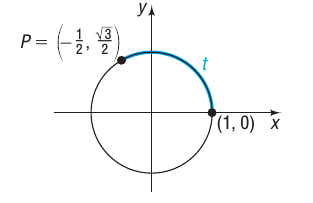
\includegraphics[width=10cm,keepaspectratio=true]{./trig/sull0619.png}
		% sull0618.png: 0x0 pixel, 300dpi, 0.00x0.00 cm, bb=
		\label{fig:0619}
	\end{figure}

{}
	\begin{problema}
		Sea $t$ un número real y $P=\left(\dfrac{\sqrt{3}}{2}, \dfrac{1}{2} \right)$
		un punto en el círculo unitario que corresponde a $t$. Encuentre los valores de las seis funciones trigonométricas.
	\end{problema}
	

\subsection{Funciones trigonométricas de ángulos}
{}
	\begin{figure}[h]
		\centering
		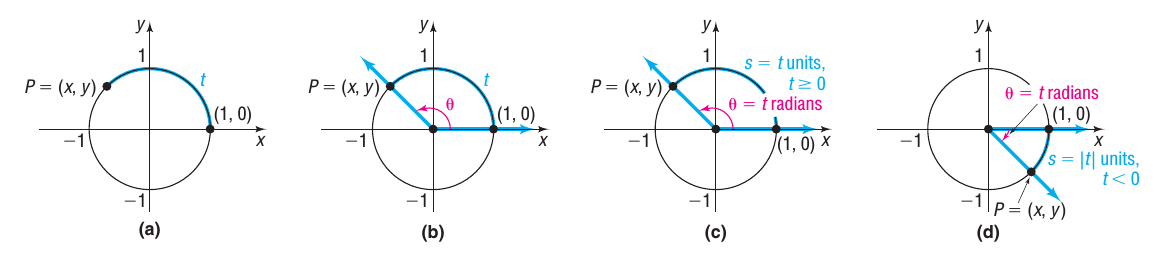
\includegraphics[width=10cm,keepaspectratio=true]{./trig/sull0620.png}
		% sull0618.png: 0x0 pixel, 300dpi, 0.00x0.00 cm, bb=
		\label{fig:0620}
	\end{figure}

{}
	Entonces, podemos definir una función trigonométrica en ángulos siempre y cuando este medido en radianes:
	\begin{align*}
		f(\theta)=f(t \texttt{ radianes})
	\end{align*} si $\theta= t \texttt{ radianes}$.

{}
	\begin{problema}
		\label{exmp:sull0602}
		Encuentre el valor exacto de las seis funciones trigonométricas en:
		\begin{itemize}
			\item $\theta=0=0^{o}$
			\item $\theta=\frac{\pi}{2}=90^{o}$ 
			\item $\theta=\pi=180^{o}$ 
			\item $\theta=\frac{3\pi}{2}=270^{o}$
		\end{itemize}
		
	\end{problema}
	

{}
	\begin{figure}[h]
		\centering
		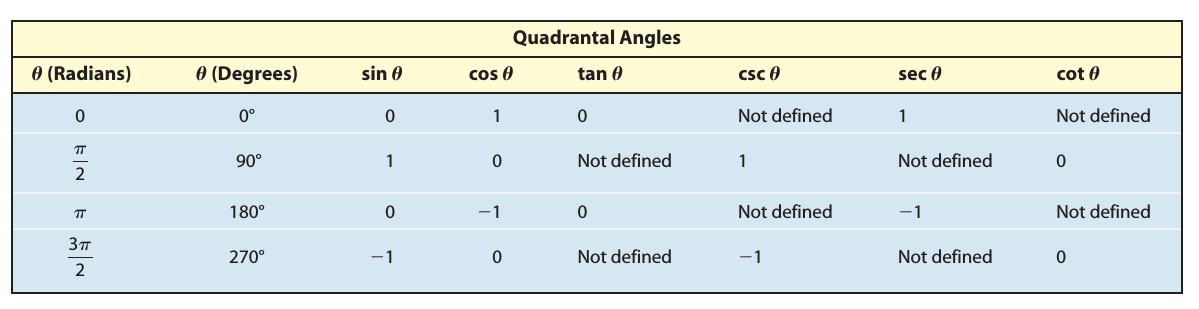
\includegraphics[width=11cm,keepaspectratio=true]{./trig/sull06t2.png}
		% sull06t2.png: 0x0 pixel, 300dpi, 0.00x0.00 cm, bb=
		\label{fig:06t2}
	\end{figure}
	

{}
	\begin{problema}
		\label{exmp:sull0603}
		Encuentre el valor exacto de:
		\begin{itemize}
			\item $\sin(3\pi)$ 
			\item $\cos(-270^{o})$
		\end{itemize}
	\end{problema}
	

{}
	\begin{problema}
		\label{exmp:sull0604}
		Encuentre el valor exacto de las seis funciones trigonométricas en $\frac{\pi}{4}=45^{o}$.
	\end{problema}
	

{Valor exacto en $\frac{\pi}{4}$}
	\begin{problema}
		\label{exmp:sull0605}
		Encuentre el valor exacto de cada expresión:
		\begin{itemize}
			\item $\sin(45^{o})\cos(180^{o})$
			\item $\tan\left( \frac{\pi}{4} \right)-\sin\left( \frac{3\pi}{2} \right)$
			\item $\left( \sec\frac{\pi}{4} \right)^{2}+\csc\frac{\pi}{2}$
		\end{itemize}
		
	\end{problema}
	

{Valor exacto en $\frac{\pi}{6}$ y $\frac{\pi}{3}$}
	\begin{figure}[h]
		\centering
		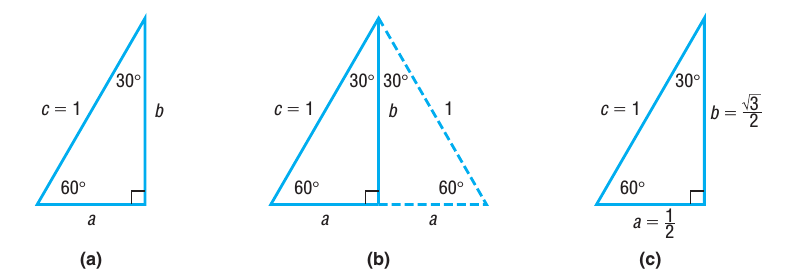
\includegraphics[width=10cm,keepaspectratio=true]{./trig/sull0624.png}
		% sull0624.png: 0x0 pixel, 300dpi, 0.00x0.00 cm, bb=
		\label{fig:0624}
	\end{figure}
	

{}
	\begin{problema}
		\label{exmp:0606}
		Encuentre el valor exacto de las seis funciones trigonométricas de $\frac{\pi}{3}=60^{o}$.
	\end{problema}
	

{}
	\begin{problema}
		\label{exmp:0607}
		Encuentre el valor exacto de las seis funciones trigonométricas de $\frac{\pi}{6}=30^{o}$.
	\end{problema}
	

{}
	\begin{figure}[h]
		\centering
		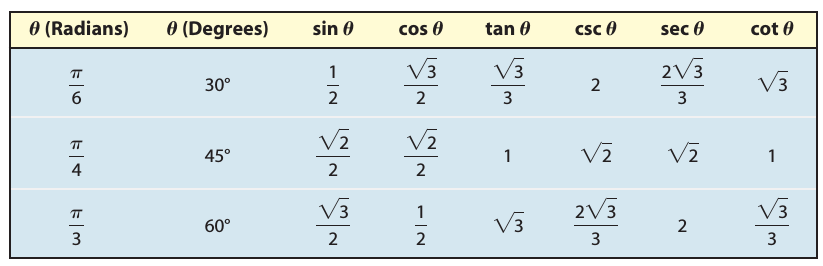
\includegraphics[width=11cm,keepaspectratio=true]{./trig/sull06t3.png}
		% sull06t3.png: 0x0 pixel, 300dpi, 0.00x0.00 cm, bb=
		\label{fig:tab3}
	\end{figure}
	

{}
	\begin{problema}
		Un recolector de lluvia se construye a partir de planchas de aluminio de 12 pulgadas de ancho. Después de marcar 4 pulgadas a partir de cada extremo, está longitud se dobla a un ángulo $\theta$. Encuentre el área transversal máxima del recolector. 
	\end{problema}


	\begin{figure}[h]
		\centering
		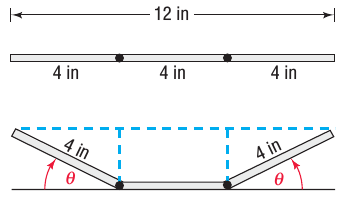
\includegraphics[width=10cm,keepaspectratio=true]{./trig/sull0627.png}
		% sull0627.png: 0x0 pixel, 300dpi, 0.00x0.00 cm, bb=
		\label{fig:0627}
	\end{figure}



\section{Funciones trigonométricas inversas}

\subsection{Funciones inversas}
{}
	Sea $f:A\to B$ una función. Diremos que $f$ es \emph{invertible} si para cada $y\in B$ \emph{siempre} corresponde un \emph{único} $x\in A$, tal que
	\begin{align*}
		f(x)=y.
	\end{align*}

{}
	Si una función $f$ es invertible, entonces existe una función $g:B\to A$ tal que $y=f(x)$ si y solo si $g(y)=x$.  En otras palabras, podemos despejar $x$.  Es usual denotar a tal función $g$ por $f^{-1}$ y llamarle \emph{inversa de $f$}.

{Propiedades del inversa}
	\begin{itemize}
		\item $f^{-1}\left( f(p) \right)$ para todo $p\in A.$ 
		\item $f\left( f^{-1}(p) \right)$ para todo $p\in B.$ 
		\item $\texttt{Dominio}(f)=\texttt{Rango}(f^{-1})$ y viceversa. 
		\item La gráfica de $f^{-1}$ es la reflexión a $45^{o}$ de la gráfica de $f$.
	\end{itemize}
	

% \subsection{Seno inverso}
% {}
% \begin{figure}[h]
%  \centering
%  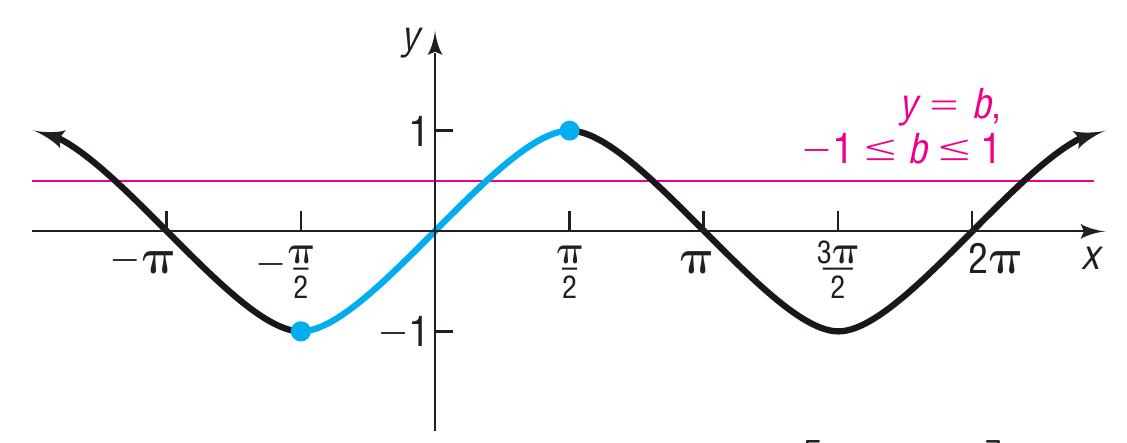
\includegraphics[width=11cm,keepaspectratio=true]{./trig/sull0701.png}
%  % sull0701.png: 0x0 pixel, 300dpi, 0.00x0.00 cm, bb=
%  \label{fig:0701}
%  \caption{$y=\sin(x), -\infty<x<\infty, -1\leq y \leq 1$}
% \end{figure}
% 
% 
% {}
% \begin{figure}[h]
%  \centering
%  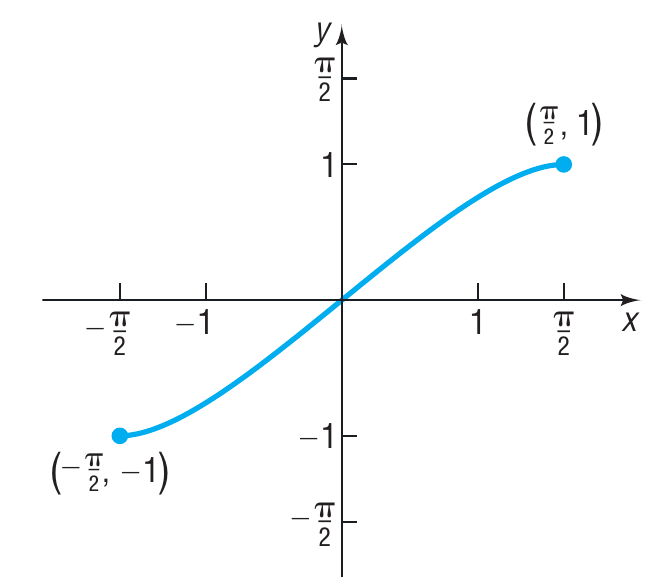
\includegraphics[height=7cm,keepaspectratio=true]{./trig/sull0702.png}
%  % sull0702.png: 0x0 pixel, 300dpi, 0.00x0.00 cm, bb=
%  \caption{$y=\sin(x), -\frac{\pi}{2}\leq x \leq \frac{\pi}{2}, -1\leq y \leq 1$}
%  \label{fig:0702}
% \end{figure}
% 
% 
% {}
% \begin{figure}[h]
%  \centering
%  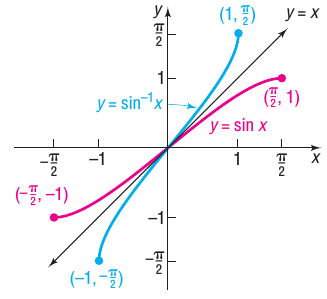
\includegraphics[height=6cm,keepaspectratio=true]{./trig/sull0703.png}
%  % sull0703.png: 0x0 pixel, 300dpi, 0.00x0.00 cm, bb=
%  \caption{$y=\sin^{-1}x, -1\leq x \leq 1, -\dfrac{\pi}{2}\leq y \leq \dfrac{\pi}{2}$}
%  \label{fig:0703}
% \end{figure}
% 
% 
% {Seno inverso}
% $$
% y = \sin^{-1} \iff
% \begin{cases}
%  x=\sin(y)\\
%  -1 \leq x \leq 1 \\
%  -\dfrac{\pi}{2} \leq y \leq \dfrac{\pi}{2}
% \end{cases}
% $$
% 
% {}
% \begin{problema}
%  Encuentre el valor exacto de
%  \begin{itemize}
%   \item $\sin^{-1}(1)$ 
%   \item $\sin^{-1}(0)$ 
%   \item $\sin^{-1}\left( -\frac{1}{2} \right)$ 
%   \item $\sin^{-1}\left( \frac{\sqrt{2}}{2} \right)$
%  \end{itemize}
% 
% \end{problema}
% 
% 
% {}
% \begin{problema}
%  Encuentre el valor exacto de 
%  \begin{itemize}
%   \item $\sin^{-1}\left( \sin\left( \frac{\pi}{8} \right) \right)$
%   \item $\sin^{-1}\left( \sin\left( \frac{5\pi}{8} \right) \right)$
%  \end{itemize}
% 
% \end{problema}
% 
% 
% {}
% \begin{problema}
%  Encuentre el valor exacto de 
%  \begin{itemize}
%   \item $\sin\left( \sin^{-1}(0.5) \right)$ 
%   \item $\sin\left( \sin^{-1}(1.8) \right)$ 
%   \item $\sin\left( \sin^{-1}\left( \frac{1}{4} \right) \right)$
%  \end{itemize}
% 
% \end{problema}
% 
% 

% \subsection{Coseno inverso}
% {}
% \begin{figure}[h]
%  \centering
%  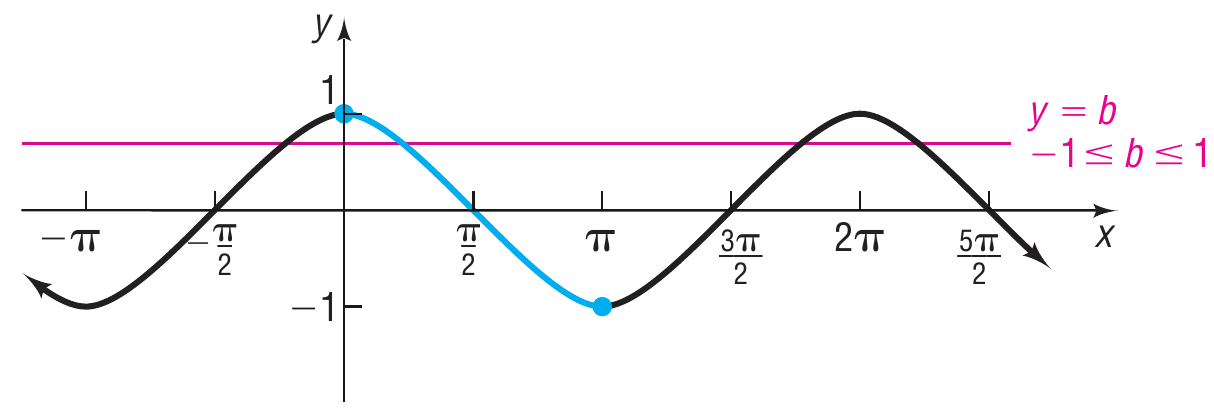
\includegraphics[width=10cm,keepaspectratio=true]{./trig/sull0707.png}
%  % sull0707.png: 0x0 pixel, 300dpi, 0.00x0.00 cm, bb=
%  \caption{$y=\cos(x),-\infty < x <\infty, -1\leq y \leq 1$}
%  \label{fig:0707}
% \end{figure}
% 
% 
% {}
% \begin{figure}[h]
%  \centering
%  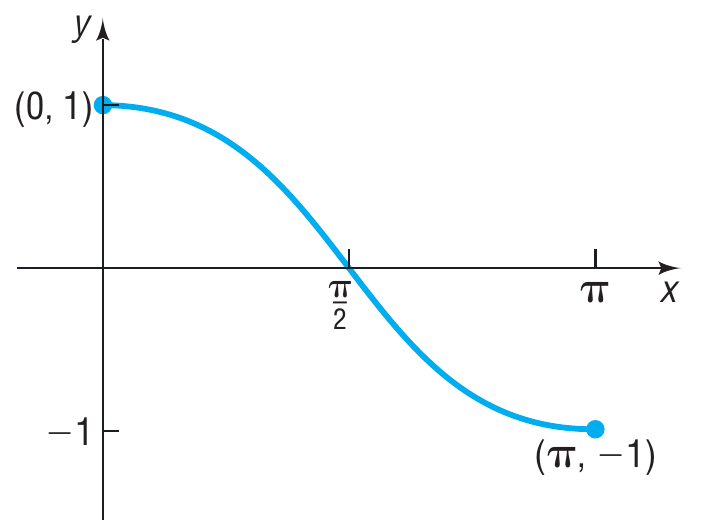
\includegraphics[width=10cm,keepaspectratio=true]{./trig/sull0708.png}
%  % sull0708.png: 0x0 pixel, 300dpi, 0.00x0.00 cm, bb=
%  \caption{$y=\cos(x),0 \leq x \leq \pi, -1\leq y \leq 1$}
%  \label{fig:0708}
% \end{figure}
% 
% 
% {}
% \begin{figure}[h]
%  \centering
%  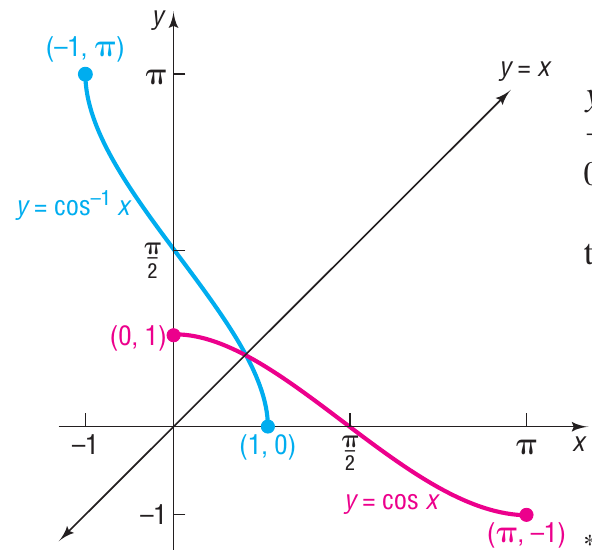
\includegraphics[width=7cm,keepaspectratio=true]{./trig/sull0709.png}
%  % sull0709.png: 0x0 pixel, 300dpi, 0.00x0.00 cm, bb=
%  \caption{$y=\cos(x), -1\leq x \leq 1, 0\leq y \leq \pi$}
%  \label{fig:0709}
% \end{figure}
% 
% 
% {Coseno inverso}
% $$y=\cos^{-1}(x)\iff
% \begin{cases}
%  x=\cos(y) \\
%  -1\leq x \leq 1 \\
%  0 \leq y \leq \pi
% \end{cases}
% $$
% 
% {}
% \begin{problema} Encuentre el valor exacto de
%  \begin{itemize}
%   \item $\cos^{-1}(0)$ 
%   \item $\cos^{-1}\left( -\frac{\sqrt{2}}{2} \right)$
%  \end{itemize}
% 
% \end{problema}
% 
% 
% {}
% \begin{problema}
%  Encuentre el valor exacto de:
%  \begin{itemize}
%   \item $\cos^{1}\left( \cos\frac{\pi}{12} \right)$
%   \item $\cos\left( \cos^{-1}(-0.4) \right)$ 
%   \item $\cos^{-1}\left( \cos\left( -\frac{2\pi}{3} \right) \right)$ 
%   \item $\cos\left( \cos^{-1}\pi \right)$
%  \end{itemize}
% 
% \end{problema}
% 
% 

\subsection{Tangente inversa}
{}
	\begin{figure}[h]
		\centering
		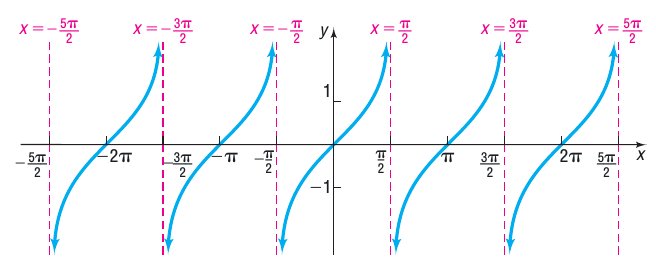
\includegraphics[width=10cm,keepaspectratio=true]{./trig/sull0712.png}
		% sull0712.png: 0x0 pixel, 300dpi, 0.00x0.00 cm, bb=
		\label{fig:0712}
		\caption{$y=\tan(x)$}
	\end{figure}
	

{}
	\begin{figure}[h]
		\centering
		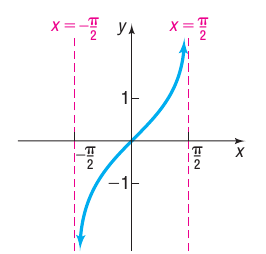
\includegraphics[height=7cm,keepaspectratio=true]{./trig/sull0713.png}
		% sull0713.png: 0x0 pixel, 300dpi, 0.00x0.00 cm, bb=
		\caption{$y=\tan(x), \; -\frac{\pi}{2}<x<\frac{\pi}{2}, \; 
			-\infty < x < \infty$}
		\label{fig:0713}
	\end{figure}
	

{}
	\begin{figure}[h]
		\centering
		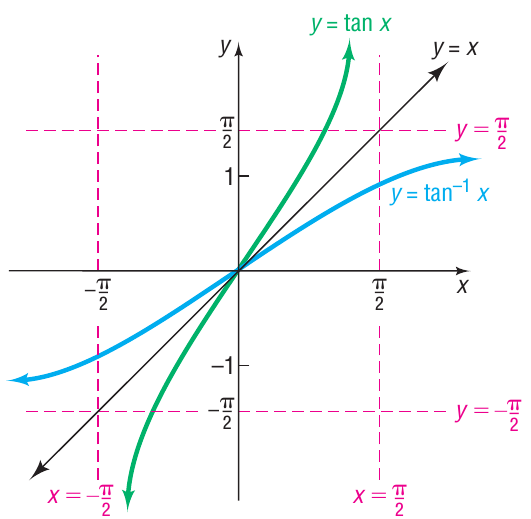
\includegraphics[height=7cm,keepaspectratio=true]{./trig/sull0714.png}
		% sull0714.png: 0x0 pixel, 300dpi, 0.00x0.00 cm, bb=
		\label{fig:0714}
	\end{figure}
	

{}
	\begin{figure}[h]
		\centering
		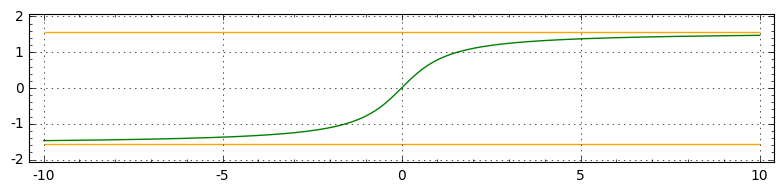
\includegraphics[width=10cm,keepaspectratio=true]{./trig/arctan.png}
		% arctan.png: 0x0 pixel, 300dpi, 0.00x0.00 cm, bb=
		\caption{$y=\tan^{-1}(x)$}
		\label{fig:arctan}
	\end{figure}

{Tangente inversa}
	$$y=\tan^{-1}(x)\iff
	\begin{cases}
		x=\tan(y)\\
		-\infty < x < \infty \\
		-\dfrac{\pi}{2} < y < \dfrac{\pi}{2}
	\end{cases}
	$$


{}
	\begin{problema}
		Encuentre el valor exacto de
		\begin{itemize}
			\item $\tan^{-1} 1$ 
			\item $\tan(-\sqrt{3})$ 
			\item $\tan^{-1}0$ 
			\item $\tan^{-1}\left( \tan\frac{4\pi}{5} \right)$
		\end{itemize}
		
	\end{problema}


\subsection{Vectores}
{}
	Diremos que un vector $\langle x,y \rangle$ esta en su \emph{forma polar (estándar)} ${\color{red}r\exp(\theta i)}$ si 
	\begin{align*}
		x =& r\cos(\theta)\\
		y =& r\sin(\theta)
	\end{align*} con $-\pi < \theta \leq \pi$.

{}
	\begin{center}
		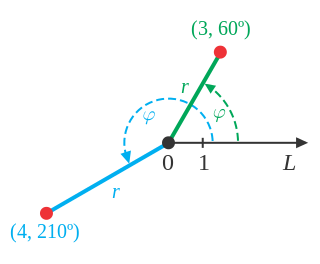
\includegraphics[height=5cm,keepaspectratio=true]{./trig/Examples_of_Polar_Coordinates.png}
		% Examples_of_Polar_Coordinates.svg.png: 0x0 pixel, 300dpi, 0.00x0.00 cm, bb=
	\end{center}
	

{}
	\begin{problema}
		Escriba los siguientes vectores en su forma polar (estándar):
		\begin{itemize}
			\item $\langle 1, \sqrt{3}\rangle$ 
			\item $\langle 1, -\sqrt{3}\rangle$ 
			\item $\langle -1, \sqrt{3}\rangle$ 
			\item $\langle -1, -\sqrt{3}\rangle$ 
		\end{itemize}
		
	\end{problema}
	

\subsection{Optimización}

	\begin{problema}
		\label{exe:0776}
		Suponga que en una sala de cine, una pantalla tiene 28 pies de alto. Cuando un espectador se sienta, la parte inferior de la pantalla tiene una altura de 6 pies por encima de su nivel de visión. El ángulo formado al dibujar una linea desde la parte inferior de la pantalla a la parte superior se conoce como ángulo de visión. Encuentre el ángulo máximo de visión respecto a la distancia al muro que sostiene la pantalla.
	\end{problema}


{}
	\begin{figure}[h]
		\centering
		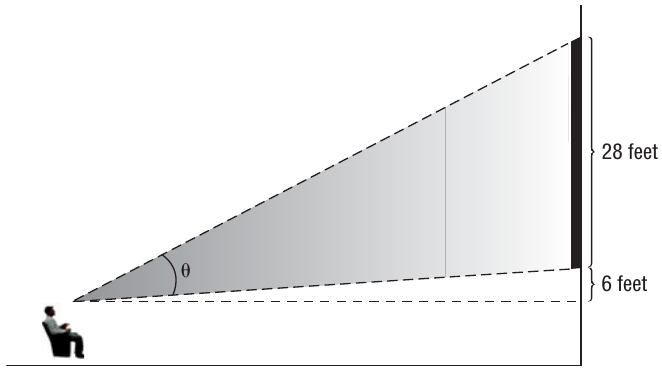
\includegraphics[width=10cm]{./trig/angulo_vision.png}
		% angulo_vision.png: 0x0 pixel, 300dpi, 0.00x0.00 cm, bb=
		\caption{Ángulo de visión}
		\label{fig:angulo_vision}
	\end{figure}
	

{Sugerencia}
	\begin{align*}
		\dfrac{d}{dx}\left( \tan^{-1}\left( \dfrac{A}{x} \right) \right)=
		-\dfrac{A}{A^{2}+x^{2}}
	\end{align*}

